\chapter{Metamodel dla języka CAL}\label{chapter:cal-metamodel}

Aby otrzymać graficzny edytor modeli wykorzystując \SiriusWeb{} należy
najpierw zaprojektować metamodel \EMF{} opisujący strukturę modeli oraz ich
reprezentację graficzną, która później będzie możliwa do modyfikacji przez
użytkowników. W tym rozdziale
zostanie omówiony język \emph{\acrfull{CAL}} służący do opisu obliczeń w
systemie \BalticLSC{}, a~następnie omówiony zostanie przygotowany metamodel
\EMF{}.

\section{Język opisu obliczeń w BalticLSC}

Obliczenia rozproszone wykonywane przez system \BalticLSC{} są zapisywane w
formie \emph{aplikacji obliczeniowej}
(\emph{\selectlanguage{english}computation application})
korzystając ze składni języka \emph{\acrfull{CAL}} przygotowanego dla tego
właśnie systemu.

Podstawowym obiektem, który wysyła (wyjście)
% TODO: zmienić port -> pin w całej pracy
lub odbiera (wejście) dane, jest \emph{port}. Jest on reprezentowany za pomocą
ikony kwadratu ze strzałką skierowaną w prawą stronę. Aplikacja obliczeniowa
składa
się z modułów obliczeniowych posiadających swoje porty, portów samej aplikacji
obliczeniowej, oraz połączeń między tymi portami. Grot połączenia wskazuje
kierunek przepływu danych.
Porty aplikacji obliczeniowej są zaznaczone na
diagramie ikoną portu (strzałką skierowaną w prawo) z pogrubioną
jedną z krawędzi ikony --- lewą dla wejścia, prawą dla wyjścia.

Porty modułów oraz aplikacji obliczeniowych mają różne ikony, które
są ustalane na~podstawie ich właściwości. Są dwa kryteria wpływające na ikonę:

\begin{itemize}
	\item krotność danych, które obsługuje port (\emph{data
		      multiplicity}):  dla pojedynczego pliku będzie to~pojedyncza strzałka, a dla katalogu --- wiele strzałek,
	\item liczba pakietów przyjmowanych lub wysyłanych danych (\emph{token
		      multiplicity}, czy oczekuje pojedynczego zestawu danych wejściowych, czy moduł obsłuży kolejne zestawy danych wysyłane po chwili bez ponownego uruchomienia).
\end{itemize}

Moduł obliczeniowy rozpoczyna obliczenia dopiero gdy na każdym jego wejściu
znajdują się dane.

Przykładowe aplikacje obliczeniowe zostały przedstawione na
rysunkach~\ref{rys:sekwencyjna-aplikacja-obliczeniowa}
i~\ref{rys:mozliwa-do-zrownoleglenia-aplikacja-obliczeniowa}.
Pierwsza z nich (rysunek~\ref{rys:sekwencyjna-aplikacja-obliczeniowa}) jest
aplikacją, w której obliczenia mogą zostać wykonane
wyłącznie sekwencyjnie, ponieważ dane przepływają sekwencyjnie od wejścia
kolejno przez moduły nazwane \texttt{VideoToFrames}, \texttt{Face Detector},
\texttt{Blur Module}, \texttt{Blur module}, aż w końcu trafiają do wyjścia.
Inna jest struktura aplikacji na
rysunku~\ref{rys:mozliwa-do-zrownoleglenia-aplikacja-obliczeniowa}. Tam
przepływ danych rozdziela się~po~module obliczeniowym \texttt{Pdf page
	splitter} i obliczenie modułów \texttt{OCT Tesseract Tess 0.1} oraz
\texttt{OCR Tesseract LSTM 0.1} może zostać wykonane równolegle, być może
przez różne węzły obliczeniowe. Ich wyniki trafią później do modułu \texttt{Pdf
	data joiner 0.1} i przejdą dalej przez pozostałe moduły w sposób
sekwencyjny.

% \begin{noindent}
\begin{figure}[!ht]
	\centering

	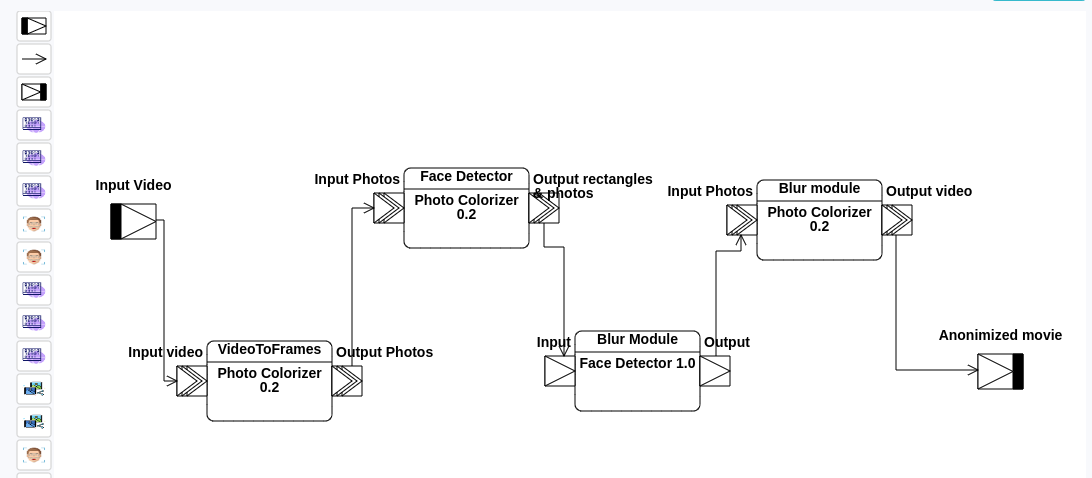
\includegraphics[width=0.95\linewidth]{./images/balticlsc-example-diagram.png}
	\caption{Aplikacja obliczeniowa w \BalticLSC{} z obliczeniami
		sekwencyjnymi}\label{rys:sekwencyjna-aplikacja-obliczeniowa}
	\medskip
	{\small Źródło: aplikacja obliczeniowa \emph{Pdf to readable pdf converter} z
		systemu \emph{BalticLSC},\\
    % NOTE: to nie może być \footnote, Latex wyrzuca wtedy błąd
		\url{https://balticlsc.iem.pw.edu.pl/#/computation-application/5532b8b8-a39c-4725-8880-80ec5b2207a4}
  }
\end{figure}
% \end{noindent}

% \begin{noindent}
\begin{figure}[!ht]
	\centering

	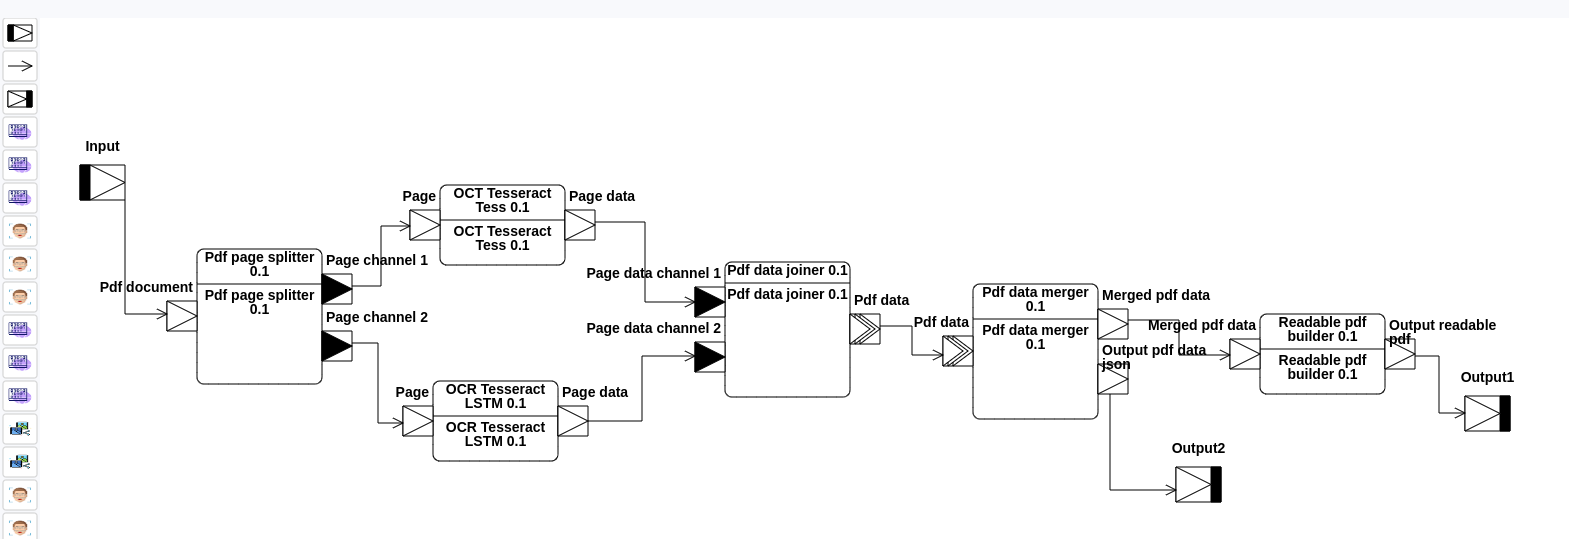
\includegraphics[width=0.99\linewidth]{./images/balticlsc-concurrent-application-example.png}
	\caption{Aplikacja obliczeniowa w \BalticLSC{} z możliwością
		zrównoleglenia obliczeń}\label{rys:mozliwa-do-zrownoleglenia-aplikacja-obliczeniowa}
  \medskip
  {\small Źródło: aplikacja obliczeniowa \emph{Movie test}
    z systemu \emph{BalticLSC},\\
    \url{https://balticlsc.iem.pw.edu.pl/#/computation-application/27571955-6e2b-4735-85ea-44f5438ca7f6}}
\end{figure}
% \end{noindent}

\section{Stworzony metamodel EMF dla języka CAL}

% TODO: zmienić metamodel EMF dla języka CAL -> metamodel w formacie ECore
% przygotowany dla języka CAL. Wprowadzić zmiany w całej pracy magisterskiej

Przygotowany metamodel \EMF{} dla języka \CAL{} widoczny jest na
rysunku~\ref{rys:cal-emf-metamodel}.
% TODO: wyjaśnić dlaczego na rysunku z metamodelem CAL w ECore są ikony dla
% niektórych klas
Bazuje on~na metamodelu
opracowanym w ramach projektu \BalticLSC{}~\cite{cal-metamodel}, który widoczny
jest na~rysunku~\ref{rys:cal-metamodel-balticlsc}.
Na potrzeby edytora diagramów nie są potrzebne wszystkie elementy oryginalnego
metamodelu. Niektóre klasy i właściwości zostały pominięte, ponieważ nie były
istotne z~perspektywy edycji diagramu.

% TODO: napisać że niektóre klasy są nowe lub mają inne znaczenie i zostanie to
% wyjaśnione w dalszej części tekstu

% TODO: napisać, że te diagramy przedstawiają jedynie składnię abstrakcyjną
% metamodelu, czyli jego strukturę. Składnia konkretna zostanie omówiona wraz z
% elementami modelu, a widoczna jest na obrazku rys 13.

\begin{figure}[!hb]
	\centering

	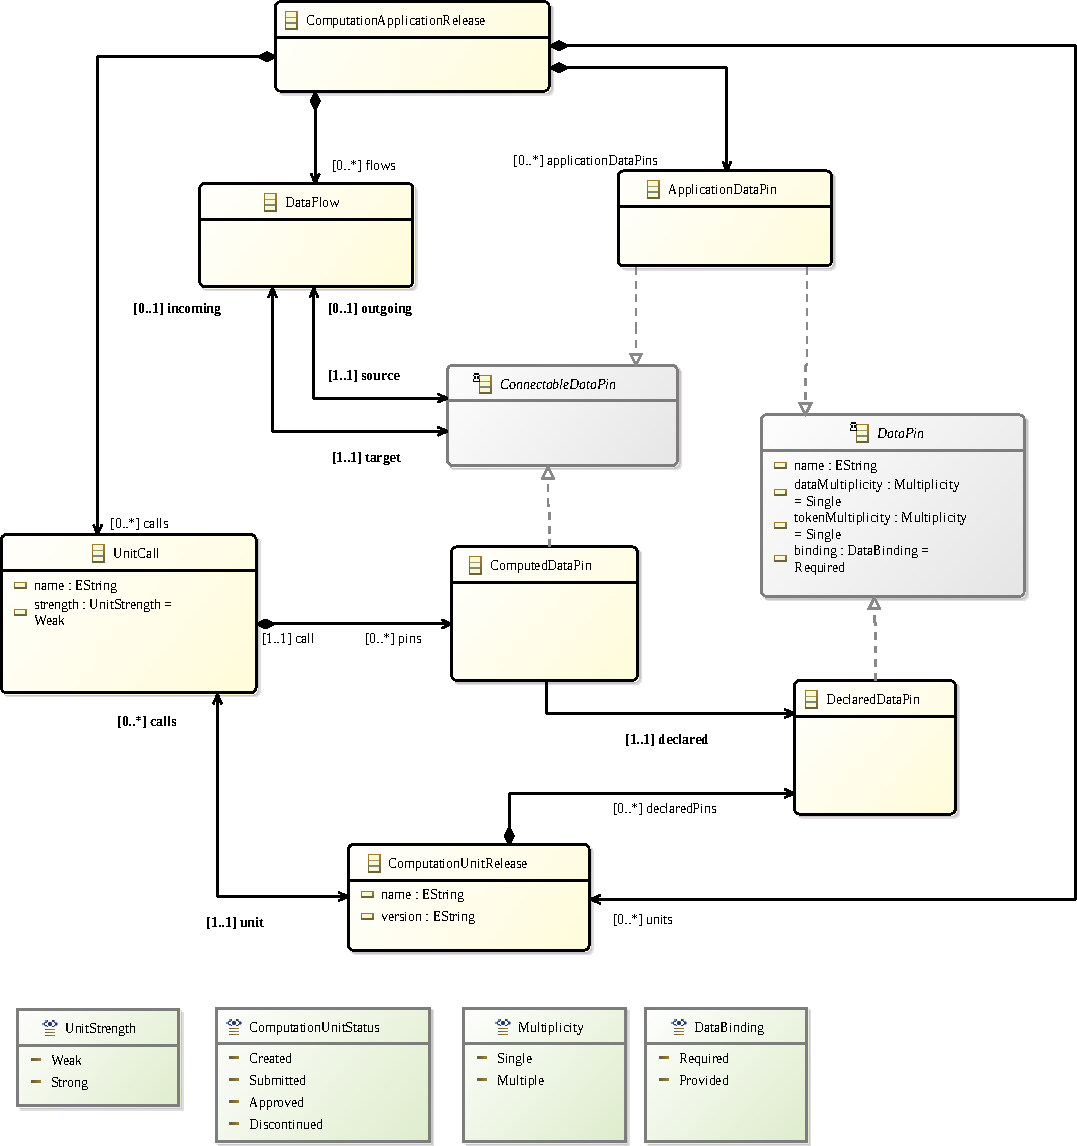
\includegraphics[width=0.92\linewidth]{./images/cal-emf-metamodel.pdf}
	\caption{Metamodel \EMF{} języka \CAL{} przygotowany w
		ramach tej pracy}\label{rys:cal-emf-metamodel}
\end{figure}

\begin{figure}[!ht]
	\centering

	% NOTE: this image is pretty tall, so it must be kept much smaller than the
	% line width so it does not take up the whole page, moving all incoming
	% images to the bottom of the chapter.

	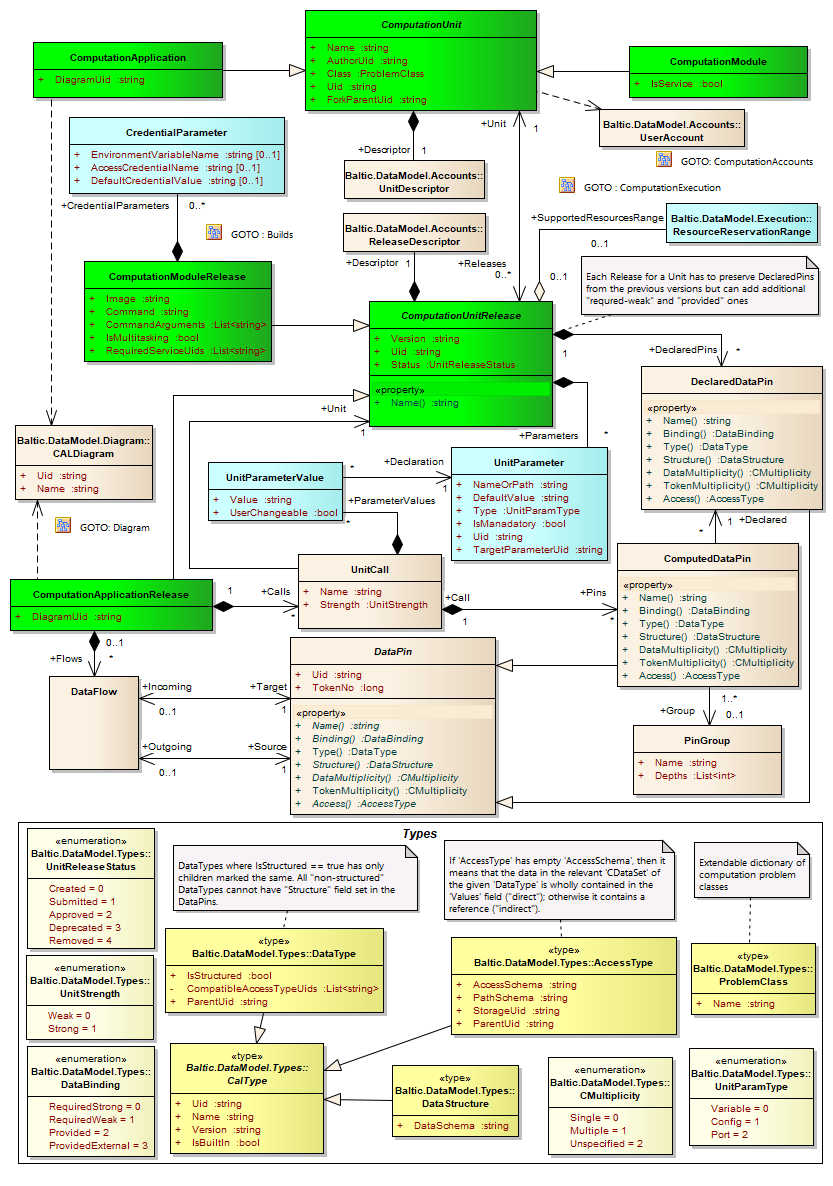
\includegraphics[width=0.82\linewidth]{./images/cal-metamodel-balticlsc.png}
	\caption{Metamodel języka \CAL{} używany w projekcie
		\BalticLSC{}}\label{rys:cal-metamodel-balticlsc}

	\medskip
	{\small Źródło:
		\url{https://www.balticlsc.eu/model/index.htm?goto=4:2:404}}
\end{figure}

Model w \EMF{} ma strukturę grafową. Głównym jego elementem jest obiekt typu
\texttt{Computation\-Application\-Release}, który odpowiada całemu diagramowi
(aplikacji obliczeniowej). Nie~ma~on~własnych właściwości. Zawiera on w sobie
natomiast 4 typy obiektów:

\begin{itemize}
	\item \texttt{ComputationUnitRelease} --- są to obiekty odpowiadające
	      rodzajom modułów i aplikacji obliczeniowych dostępnych w systemie \BalticLSC{} i opisują ich właściwości.

	      Oprócz informacji o nazwie i wersji modułu zawierają w sobie obiekty \texttt{DeclaredDataPin} dziedziczące z \texttt{DataPin}, które opisują porty tego modułu obliczeniowego.

	      Obiekty te nie są wyświetlane na diagramie (nie występują w wizualnej reprezentacji modelu). Można je zobaczyć jedynie w drzewie obiektów modelu.

	      % TODO: Wyjaśnić dlaczego tutaj ComputationUnitRelease zawiera
	      % jednocześnie moduły i aplikacje obliczeniowe, a w CAL jest inaczej.

	\item \texttt{UnitCall} --- wywołania dostępnych modułów
	      obliczeniowych. Każdy dostępny moduł obliczeniowy może zostać wywołany dowolną liczbę razy. Każde wywołanie to osobny obiekt \texttt{UnitCall} ze wskazaniem modułu, który ma zostać wywołany, a także z obiektami \texttt{ComputedDataPin}, które reprezentują porty tego modułu.

	      Taka reprezentacja pozwala na zapisanie szczegółów dotyczących dostępnych modułów obliczeniowych wyłącznie raz w modelu, a później wskazywanie tych elementów w~każdym z wywołań modułu.

	      Rozwiązanie to ma jednak pewne ograniczenie --- aby oznaczyć wywołanie modułu za~pomocą obiektu \texttt{UnitCall}, należy najpierw stworzyć obiekt \texttt{Computation\-Unit\-Release} i~dodać odpowiednie \texttt{Declared\-Data\-Pin}. Można wywołać jedynie moduły, które są~zapisane w metamodelu. Sam metamodel nie ma możliwości pobrania informacji o~dostępnych modułach obliczeniowych z systemu \BalticLSC{}, więc w podstawowej wersji metamodelu to użytkownik musi samemu dodać dostępne moduły w metamodelu.

	      Na diagramie obiekty te są reprezentowane jako prostokąty ze swoimi portami umieszczonymi na krawędziach. Wewnątrz prostokąta znajduje się etykieta zawierająca nazwę umożliwiającą wyróżnienie tego konkretnego wywołania modułu, oraz nazwę i wersję wydania wywoływanego modułu. % TODO: odnieść się do obrazka pokazującego przykładowy diagram

	\item \texttt{ApplicationDataPin} --- porty aplikacji obliczeniowej
	      opisywanej przez ten model. Są~to~wejścia i wyjścia z diagramu. Właściwości portu są dziedziczone z klasy \texttt{DataPin}.

	      % TODO: opisać dlaczego taki obiekt został wprowadzony i nie użyto
	      % DeclaredDataPin bezpośrednio

	      Z uwagi na fakt, że te porty będą łączone z innymi portami, klasa ta dziedziczy z klasy \texttt{ConnectableDataPin}.

	      Na diagramie obiekty te reprezentowane są jako prostokąty z ikoną strzałki w prawo z~pogrubionym prawym lub lewym jej bokiem.

	      % TODO: odnieść się do obrazka pokazującego przykładowy diagram

	\item \texttt{DataFlow} --- połączenia między portami
	      (\texttt{ConnectableDataPin}) umieszczonymi na~wywołaniach węzłów
	      obliczeniowych (\texttt{ComputedDataPin} na \texttt{UnitCall}) lub portami aplikacji obliczeniowej (\texttt{ApplicationDataPin}).

	      Na diagramie obiekty te reprezentowane są jako krawędzie z grotem wskazującym kierunek przepływu danych.

	      % TODO: odnieść się do obrazka pokazującego przykładowy diagram
\end{itemize}

Przykładowy diagram reprezentujący model \EMF{} języka \CAL{} wyświetlony w
programie \SiriusDesktop{} został przedstawiony na
rysunku~\ref{rys:sirius-desktop-cal-example-model}.

% \begin{noindent}
\begin{figure}[!ht]
	\centering

	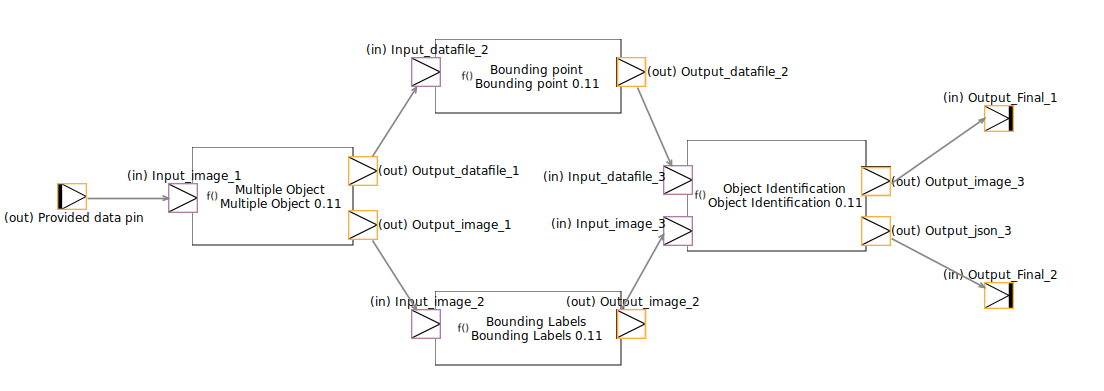
\includegraphics[width=0.95\linewidth]{./images/sirius-desktop-cal-example-model.png}
	\caption{Przykładowy diagram reprezentujący model języka \CAL{} w
		\SiriusDesktop{}}\label{rys:sirius-desktop-cal-example-model}
\end{figure}
% \end{noindent}

Oprócz podstawowej struktury metamodelu oraz jego reprezentacji w formie
diagramu zostały do niego dodane dodatkowe funkcjonalności. Zostały one opisane
w kolejnych sekcjach.

\subsection{Warunkowa zmiana stylu elementów}

% \begin{noindent}
Użytkownik może wywnioskować dodatkowe informacje z diagramu jeżeli jego wygląd
będzie zależał od właściwości elementów modelu. Takie rozwiązanie zastosowano
dla dwóch elementów metamodelu dzięki wykorzystaniu \emph{Style
	Customizations}~\cite{sirius-desktop-documentation-style-customizations}
w \EMF{}.
% \end{noindent}
Funkcjonalność ta pozwala na wskazanie za pomocą języka \AQL{} w jakich
sytuacjach styl elementu powinien zostać zmieniony, a następnie wskazać które
właściwości powinny ulec zmianie oraz ich nowe wartości.

Pierwszy styl warunkowy został użyty dla portów w metamodelu. Porty
(\texttt{DataPin}) zmieniają ikonę na podstawie swoich krotności danych oraz
paczek danych (odpowiednio \emph{data multiplicity} i \emph{token
	multiplicity}).

Z uwagi na fakt, że oba parametry mogą mieć jedną z 2 wartości,
co daje w sumie 4~możliwości, w klasie \texttt{Services} metamodelu stworzono
metodę w języku \Java{}, która zwraca nazwę odpowiedniej ikony.
Dzięki możliwości wykorzystania języka programowania osiągnięto
zamierzony efekt za pomocą jednego stylu warunkowego, a nie 4 różnych
styli dla 4 możliwości. Kod metody zwracającej nazwę ikony dla portu
został przedstawiony w listingu~\ref{lst:getDataPinIconPath-method}.

\begin{lstlisting}[float,
    floatplacement=ht,
    language=Java,
    caption={Metoda zwracająca nazwę ikony dla portu},
    label={lst:getDataPinIconPath-method}]
public String getDataPinIconPath(EObject self) {
  if (!(self instanceof DataPin)) {
    return null;
  }

  var dataPin = (DataPin) self;
  var dataPart = dataPin.getDataMultiplicity() == Multiplicity.SINGLE ? "single-data" : "multiple-data";
  var tokenPart = dataPin.getTokenMultiplicity() == Multiplicity.SINGLE ? "single-token" : "multiple-tokens";

  return dataPart + "-" + tokenPart + ".png";
}
\end{lstlisting}

Dla portów całej aplikacji obliczeniowej (\texttt{Application\-Data\-Pin} dla
\texttt{Computation\-Application\-Release}) styl warunkowy był
rozszerzeniem tego
dla portów modułów obliczeniowych. Oprócz brania pod uwagę krotności danych
oraz
paczek danych, w tym stylu znaczenie ma ponadto kierunek portu. Porty wejściowe
mają pogrubiony pasek z lewej strony, a porty wyjściowe z prawej. Dla tych
portów występują 3 cechy od których zależy ikona, co oznacza 8 możliwości.
Dzięki wykorzystaniu metody z listingu~\ref{lst:getDataPinIconPath-method} oraz
języka \AQL{} ta funkcjonalność została zrealizowana za pomocą jednego stylu
warunkowego, zamiast 8 styli dla 8 różnych wariantów.

Drugim wykorzystanym rodzajem styli warunkowych jest zmiana koloru obramowania
portów na krawędziach modułów obliczeniowych (\texttt{ComputedDataPin}) w
zależności od~kierunku przepływu danych. Porty wejściowe (\emph{required}) mają
ramkę koloru fioletowego, a~porty wyjściowe (\emph{provided}) mają ramkę koloru
pomarańczowego. Ta funkcjonalność została zaimplementowana za pomocą jednego
stylu warunkowego.

Wyniki działania obu rodzajów styli warunkowych widoczne są na
rysunku~\ref{rys:sirius-desktop-cal-example-model}.

\subsection{Narzędzia edytora diagramów}\label{sec:cal-metamodel-tools}

W metamodelach \EMF{} można zdefiniować narzędzia wspomagające i ułatwiające
edycję modeli, a także pomagające uniknąć
błędów~\cite{sirius-desktop-documentation-tools}. Również do metamodelu języka
\CAL{} dodano takie narzędzia, które zostaną omówione w tej sekcji.

Pierwszą grupą narzędzi dodanych do metamodelu \EMF{} języka \CAL{} są
narzędzia
automatyzujące pracę użytkownika, aby ten nie musiał manualnie wykonywać
niektórych czynności, a~jednocześnie aby w modelu nie znajdowały się nieużywane
elementy.

Jednym z takich narzędzi jest automatyczne usuwanie połączeń między portami
w~momencie, gdy ten port zostaje usunięty. W przypadku portów aplikacji
obliczeniowej (\texttt{Application\-Data\-Pin}) narzędzie to zastępuje zwykłą
operację usunięcia. Dla portów wywołania modułu obliczeniowego
(\texttt{ComputedDataPin}), narzędzie to uruchamiane jest podczas usuwania tego
modułu obliczeniowego. Dzięki temu narzędziu w modelu nie pozostają połączenia
zakończone jedynie z jednej strony.

Drugim z narzędzi automatyzujących pracę jest automatyczne zarządzanie
portami wywołania modułu obliczeniowego (\texttt{ComputedDataPin}) w~momencie
wskazania lub zmiany który moduł obliczeniowy ma zostać wywołany. Zmiana
atrybutu \texttt{unit} obiektu \texttt{UnitCall} usuwa aktualnie powiązane z
nim porty (o ile jakieś istniały) i tworzy nowe na podstawie definicji modułu
obliczeniowego (\texttt{ComputationUnitRelease}) zapisanej w metamodelu,
a~także jego zdeklarowanych portów (\texttt{DeclaredDataPin}). Stworzone porty
mają
automatycznie ustawione odwołania na właściwe deklaracje portów.
Wykorzystanie tego narzędzia zostało przedstawione na
rysunku~\ref{rys:sirius-desktop-change-unit-to-call}.
Rysunek~\ref{rys:sirius-desktop-empty-unit-call} demonstruje wygląd nowo
utworzonego wywołania modułu obliczeniowego bez wskazania który moduł on
wywołuje. Po wskazaniu modułu do wywołania, piny są tworzone automatycznie, co
widać na rysunku~\ref{rys:sirius-desktop-change-unit-to-call-before}. Po
ponownej zmianie modułu obliczeniowego do wywołania, poprzednie piny są
usuwane, a na ich miejsce zostają utworzone nowe, na bazie definicji wybranego
modułu obliczeniowego, co widać na
rysunku~\ref{rys:sirius-desktop-change-unit-to-call-after}.

Narzędzie to zostało przygotowane poprzez modyfikację kodu źródłowego klas
metamodelu. Została zmieniona definicja metody zmiany wskazania na moduł do
wywołania w obiekcie \texttt{UnitCall}. Podczas wywołania tej metody usuwane są
poprzednie porty i tworzone są nowe. To zachowanie opisane jest w języku
\Java{}.

Dzięki temu narzędziu użytkownik nie musi samemu usuwać starych portów
i~tworzyć nowych podczas zmiany wywoływanego modułu. Przyśpiesza to~pracę z
metamodelem i~pomaga uniknąć błędów.

% \begin{noindent}
\begin{figure}
	\centering
	\begin{subfigure}{.3\textwidth}
		\centering
		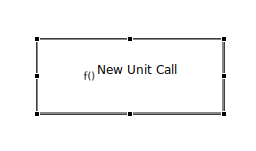
\includegraphics[width=.99\linewidth]{./images/sirius-desktop-empty-unit-call.png}
		\caption{Nowo utworzone wywołanie modułu obliczeniowego}\label{rys:sirius-desktop-empty-unit-call}
	\end{subfigure}
	\begin{subfigure}{.3\textwidth}
		\centering
		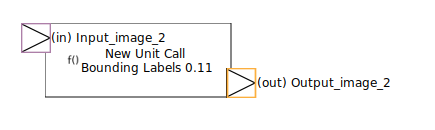
\includegraphics[width=.99\linewidth]{./images/sirius-desktop-change-unit-to-call-before.png}
		\caption{Wywołanie modułu obliczeniowego po wskazaniu modułu do
      wywołania}\label{rys:sirius-desktop-change-unit-to-call-before}
	\end{subfigure}
	\begin{subfigure}{.3\textwidth}
		\centering
		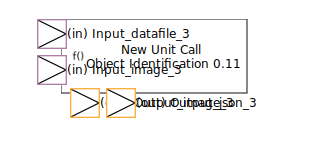
\includegraphics[width=.99\linewidth]{./images/sirius-desktop-change-unit-to-call-after.png}
		\caption{Wywołanie modułu obliczeniowego po ponownym wskazaniu modułu do
        wywołania}\label{rys:sirius-desktop-change-unit-to-call-after}
	\end{subfigure}

	\caption{Demonstracja działania narzędzia zarządzającego portami wywołań
    modułów obliczeniowych}\label{rys:sirius-desktop-change-unit-to-call}
\end{figure}
% \end{noindent}

Inną grupą narzędzi są narzędzia pomagające w przestrzeganiu poprawności
modelu. Do~tej~grupy można zaliczyć kilka narzędzi dotyczących tworzenia lub
modyfikacji połączeń między portami. Dane mogą przepływać jedynie od portów
wyjściowych do portów wejściowych. Ponadto, niemożliwe jest połączenie portów
na tym samym wywołaniu modułu obliczeniowego. Oba te wymagania mogą być
egzekwowane w modelu za pomocą narzędzi do~tworzenia połączeń (\emph{Edge
	Creation}) oraz do zmiany połączenia (\emph{Reconnect Edge}). Pierwsze
z nich za
pomocą warunków \emph{Connection Start Precondition} oraz
\emph{Connection Complete Precondition}, ustalających czy połączenie może
zostać
rozpoczęte lub zakończone w~danym elemencie, pozwala zabronić stworzenia
połączenia. Drugie z nich za pomocą warunku \emph{Precondition} ustala kiedy
zmiana jednego z końców połączenia jest możliwa.

Drugim z narzędzi w grupie pomagających w przestrzeganiu poprawności jest
narzędzie uniemożliwiające usuwanie portów wywołań modułów obliczeniowych
(\texttt{ComputedDataPin}). Są one tworzone i usuwane automatycznie podczas
wskazania modułu do wywołania i~niepoprawnym byłoby gdyby użytkownik mógł
tworzyć lub usuwać je samemu, ponieważ faktyczna liczba portów mogłaby się
wtedy nie
zgadzać z liczbą zadeklarowanych portów w~tym~module obliczeniowym.

Innym typem narzędzi są narzędzia ułatwiające tworzenie elementów modelu.
Są~3~proste narzędzia umieszczających element w modelu: dla portu wejściowego i
wyjściowego aplikacji, a także dla pustego wywołania modułu obliczeniowego, dla
którego należy później wskazać moduł, który ma wywołać. Bardziej skomplikowanym
narzędziem jest narzędzie pozwalające na~dodanie do modelu wywołania modułu
obliczeniowego, które pokazuje okno dialogowe pozwalające wybrać moduł oraz
wskazać nazwę dodawanego obiektu. Wykorzystuje ono~możliwości \SiriusDesktop{}
do tworzenia okien dialogowych (zarówno jednorazowych
jak~i~składających się z wielu
kroków)~\cite{sirius-desktop-documentation-tools} i
pozwala na dostarczeniu użytkownikowi
bardziej interaktywnych i przyjemniejszych wrażeń z pracy z modelem. Okno
dialogowe
pokazujące się po wybraniu
tego narzędzia jest przedstawione na
rysunku~\ref{rys:sirius-desktop-create-unit-call-tool}.

% \begin{noindent}
\begin{figure}[!hb]
	\centering

	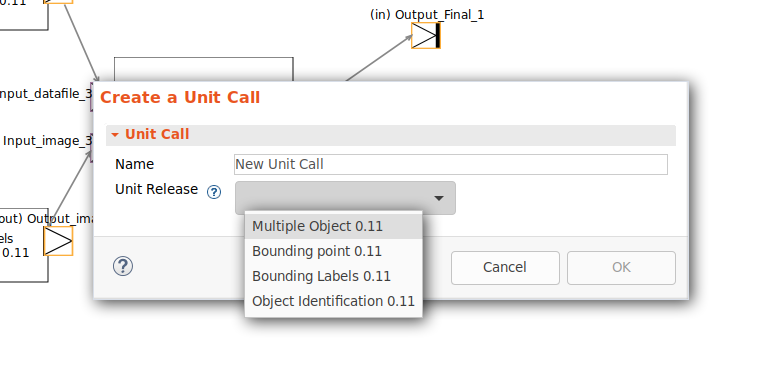
\includegraphics[width=0.95\linewidth]{./images/sirius-desktop-create-unit-call-tool.png}
	\caption{Narzędzie do interaktywnego tworzenia nowego wywołania modułu
		obliczeniowego w~\SiriusDesktop{}}\label{rys:sirius-desktop-create-unit-call-tool}
\end{figure}
% \end{noindent}

Narzędzia te uruchamiają się jedynie, gdy zmiana w modelu zostanie wykonana
poprzez edycję diagramu lub właściwości już istniejącego elementu. Podczas
bezpośredniej edycji drzewa modelu narzędzia powiązane z metamodelem są
pomijane, przez co można doprowadzić do~sytuacji, w której model nie będzie
poprawny
semantycznie. Przykładem operacji pomijającej narzędzia jest usunięcie portu
aplikacji obliczeniowej (\texttt{ApplicationDataPin}) bezpośrednio z~drzewa
modelu. Jeżeli miała ona połączenie (\texttt{DataFlow}), nie zostanie
ono~automatycznie usunięte (narzędzie, które je usuwa nie zostanie
uruchomione), co
prowadzi do istnienia w~modelu połączenia, którego jedynie jeden koniec jest
poprawnie ustawiony. Takie sytuacje natomiast są wykrywane przez reguły
walidacji strukturalnej metamodelu (połączenie musi mieć poprawne oba końce).

\subsection{Reguły walidacyjne powiązane z
	metamodelem}\label{sec:reguly-walidacyjne-metamodel}

\SiriusDesktop{} dostarcza mechanizm walidacji edytowanego modelu. Można
go uruchomić poprzez wybranie opcji \menu{Diagram > Validate} z głównego menu
programu. Wyświetlona zostanie wtedy lista informacji diagnostycznych
dotyczących modelu.

\SiriusDesktop{} domyślnie dostarcza informacji o błędach składniowych
modelu. Będą to~ostrzeżenia o braku wymaganych atrybutów lub niepoprawnej
krotności elementów (jeżeli dana właściwość powinna zawierać przykładowo co
najmniej 3 elementy, a nie więcej niż~5~elementów). Błędy te będą także
zaznaczone na diagramie za pomocą ikony czerwonego znaku \texttt{X} obok
elementu, którego wiadomość dotyczy. Zostało to zilustrowane na
rysunku~\ref{rys:sirius-desktop-syntax-validation}.
% TODO: napisać, że tylko ostatni wiersz pochodzi z walidacji składniowej, a
% reszta wierszy jest zasłonięta, ponieważ są one nieistotne z perspektywy
% walidacji składniowej (błędy edytora)
% TODO: opisać, że widoczny na liście błąd odpowiada ikonie X na diagramie
% oznaczającej błąd

% \begin{noindent}
\begin{figure}[!hb]
	\centering

	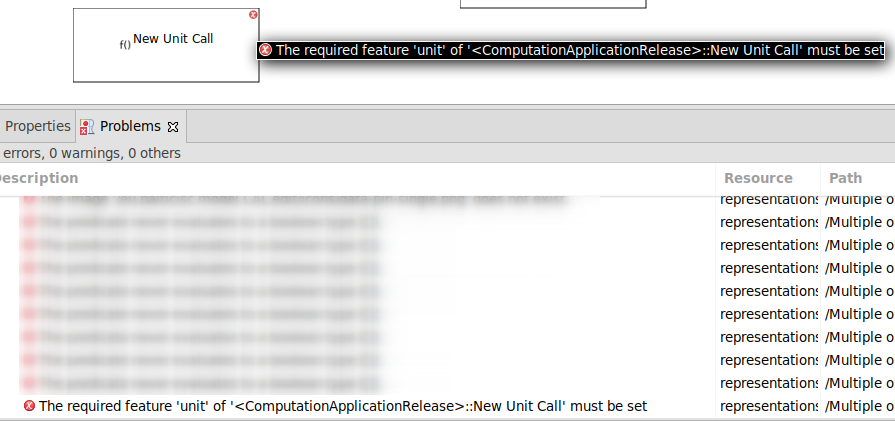
\includegraphics[width=0.95\linewidth]{./images/sirius-desktop-syntax-validation.png}
	\caption{Walidacja składniowa modeli w \SiriusDesktop{}}\label{rys:sirius-desktop-syntax-validation}
\end{figure}
% \end{noindent}

Dodatkowo w pliku \texttt{*.odesign} pakietu \texttt{.design} metamodelu można
zdefiniować \emph{Semantic Validation
	Rules}~\cite{sirius-desktop-documentation-validation-rules}.
Pozwalają one na dodanie własnych reguł walidacji semantycznej modeli. To
reguły powinny opisywać ograniczenia, których nie dostarcza opis struktury
modelu i~zależą od połączenia kilku elementów ze sobą. Można
wybrać jakich elementów reguła dotyczy, a~za~pomocą języka \AQL{} wskazać
kiedy informacja diagnostyczna powinna być pokazana, a także jaka powinna być
wiadomość wyświetlona użytkownikowi, oraz z jakim poziomem poważności
(informacja, ostrzeżenie, błąd). Jeżeli wiadomo jak można naprawić błąd, można
zdefiniować również sekwencję akcji, które będą wykonywane gdy użytkownik
wybierze
opcje automatycznego naprawiania błędów diagnostycznych.

Przykładową regułę walidacji semantycznej przedstawiono na
rysunku~\ref{rys:sirius-desktop-example-semantic-validation-rule}.
Zabrania ona~połączeń między portami znajdującymi się na tym samym wywołaniu
modułu obliczeniowego. Jej struktura wyrażona w drzewie obiektów metamodelu
jest widoczna na
rysunku~\ref{rys:sirius-desktop-example-semantic-validation-rule-tree},
a~jej~właściwości na
rysunku~\ref{rys:sirius-desktop-example-semantic-validation-rule-properties}.
Widać tam element, dla którego wiadomość zostanie wyświetlona
(\texttt{DataFlow}).
Rysunek~\ref{rys:sirius-desktop-example-semantic-validation-rule-audit}
przedstawia wyrażenie języka \AQL{}. Niespełnienie warunku spowoduje
pokazanie
informacji o błędzie. W tym przypadku sprawdza ono, czy~obiekty początkowy i
końcowy połączenia mają różnych rodziców. Nie jest to spełnione wyłącznie
jeżeli oba~porty należą do tego samego wywołania modułu obliczeniowego.
Błąd wynikający z tej reguły został
przedstawiony na
rysunku~\ref{rys:sirius-desktop-example-semantic-validation-rule-failure}.
Należało wykluczyć sytuacje, w
których połączenie jest między dwoma portami aplikacji obliczeniowej, ponieważ
takie połączenia są dozwolone.

% TODO: spróbować przenieść wcześniej, podobnie z innymi obrazkami, może się da
% bliżej tekstu
% \begin{noindent}
\begin{figure}[!hb]
	\centering
	\begin{subfigure}{.8\textwidth}
		\centering
		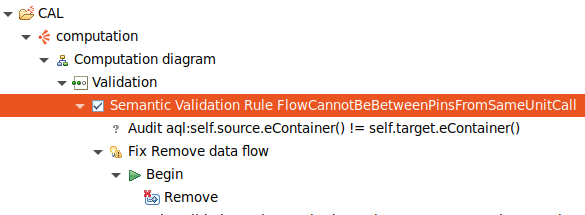
\includegraphics[width=.99\linewidth]{./images/sirius-desktop-example-semantic-validation-rule-tree.png}
		\caption{Drzewo obiektów składających się na regułę walidacji
      semantycznej}\label{rys:sirius-desktop-example-semantic-validation-rule-tree}
	\end{subfigure}

  \medskip

	\begin{subfigure}{.92\textwidth}
		\centering
		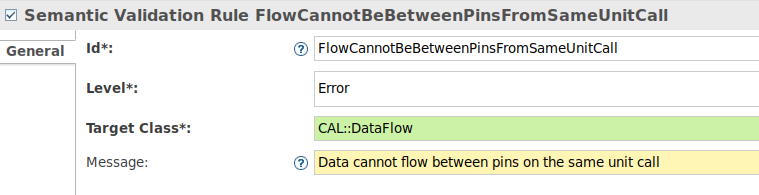
\includegraphics[width=.99\linewidth]{./images/sirius-desktop-example-semantic-validation-rule-properties.png}
		\caption{Właściwości reguły walidacji semantycznej}\label{rys:sirius-desktop-example-semantic-validation-rule-properties}
	\end{subfigure}

  \medskip

	\begin{subfigure}{.92\textwidth}
		\centering
		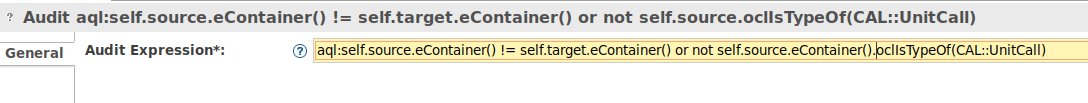
\includegraphics[width=.99\linewidth]{./images/sirius-desktop-example-semantic-validation-rule-audit.png}
		\caption{Warunek spełnienia reguły walidacji semantycznej}\label{rys:sirius-desktop-example-semantic-validation-rule-audit}
	\end{subfigure}

  \begin{subfigure}{.92\textwidth}
    \centering
    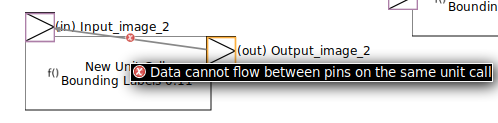
\includegraphics[width=.99\linewidth]{./images/sirius-desktop-example-semantic-validation-rule-failure.png}
    \caption{Błąd --- reguła nie została
    spełniona}\label{rys:sirius-desktop-example-semantic-validation-rule-failure}
  \end{subfigure}

	\caption{Przykładowa reguła walidacji semantycznej w \emph{Sirius
    Desktop}}\label{rys:sirius-desktop-example-semantic-validation-rule}
  \medskip
\end{figure}
% \end{noindent}

Oprócz reguły walidacji semantycznej zaprezentowanej na
rysunku~\ref{rys:sirius-desktop-example-semantic-validation-rule}
zaprojektowano 5~innych reguł informujących użytkownika o błędach w metamodelu.
Pierwsze dwie z~nich pomagają ustalić oczekiwany kierunek połączeń portów. Dla
portów oznaczonych jako wymagane (\texttt{required}) połączenie powinno być
wchodzące, a dla portów oznaczonych jako dostarczone (\texttt{provided}) ---
wychodzące. Jest to informacja niewynikająca ze struktury metamodelu, więc
została dostarczona jako reguła walidacji semantycznej. Oprócz 2 reguł
wymagających połączenia danego typu są też 2 reguły, które zabraniają
połączenia w~przeciwną stronę niż oczekiwana. Oznacza to, że jeżeli port nie
będzie miał żadnego połączenia, będzie pokazana informacja o braku, a jeżeli
dodatkowo port będzie miał połączenie w~przeciwną stronę (przykładowo, port
wymagany będzie miał połączenie wychodzące), to będą 2~wiadomości: jedna o
braku połączenia w oczekiwanym kierunku, a druga o~nieoczkiewanym połączeniu w
przeciwnym kierunku.

Ostatnią dodaną regułą jest sprawdzenie czy oba końce połączenia (obiektu
\texttt{DataFlow}) są~zdefiniowane. Jeżeli krawędź nie jest połączona z dwoma
obiektami, użytkownik dostaje o tym informacje oraz możliwość szybkiego
usunięcia takiego połączenia. Jest to szczególnie ważne, ponieważ takie
połączenia nie są pokazywane na diagramie, a jedynie wprowadzają zamieszanie w
metamodelu i utrudniają badanie jego struktury przez narzędzia, które muszą
oczekiwać, że krawędzie mogą nie być zaczepione z obu stron.

\subsection{Testy metamodelu}\label{sec:testy-metamodelu}

W sekcji~\ref{sec:cal-metamodel-tools} opisano modyfikacje kodu źródłowego klas
metamodelu, które usprawniają pracę użytkownika z modelem. Aby upewnić się, że
te modyfikacje działają poprawnie, należy je~przetestować. Można to zrobić
projektując testy
jednostkowe metamodelu w pakiecie \texttt{.tests}. \SiriusDesktop{}
automatycznie generuje kod źródłowy posiadający odpowiednią strukturę do
tworzenia testów. Dla każdego obiektu metamodelu tworzona jest osobna klasa z
jego testami.

Oprócz zwykłych plików z testami wygenerowane zostały również pliki dla
pakietów testów (\emph{\selectlanguage{english}test suite}), w których można
zdefiniować grupy testów,
które mają zostać wykonane. W~ten~sposób można podzielić testów na kilka
kategorii, na przykład testy krytyczne, testy normalne, testy o niskiej
ważności. Zgrupowanie testów pozwala na otrzymanie podsumowanego statusu
wszystkich testów w danej grupie.

Testy można później w łatwy i szybki sposób uruchomić zaznaczając pakiet z
testami w eksploratorze projektów, a później wybierając z menu głównego
\menu{Run > Run As > JUnit Test}. Uruchamiane są one wykorzystując popularny
zestaw narzędzi \JUnit{}~\cite{junit-test-tutorial}.

Posiadanie testów jednostkowych pozwala w szybszy sposób sprawdzić czy model
nadal zachowuje się zgodnie z oczekiwaniami, co jest szczególnie ważne po
modyfikacji jego kodu źródłowego lub generowaniu go na nowo po zmianach
metamodelu. Należy testować kod~zmodyfikowany lub dodany. Nie należy testować
kodu automatycznie generowanego przez \SiriusDesktop{} jeżeli nie został
on zmodyfikowany.

W ramach tej pracy magisterskiej przygotowano 2 testy jednostkowe weryfikujące
następujące zachowania dodane w kodzie źródłowym klas metamodelu:

\begin{itemize}
	\item Czy połączenia między portami usuwanych wywołań węzłów obliczeniowych są również usuwane?

	\item Czy porty są automatycznie usuwane i tworzone podczas zmiany wskazania modułu, który ma zostać wywołany w danym obiekcie \texttt{UnitCall}?

	      Weryfikowane jest czy utworzone porty mają poprawnie ustawione odwołania na~zdeklarowane porty danego modułu obliczeniowego.
\end{itemize}

Są to jedyne dwie modyfikacje kodu źródłowego metamodelu, których dokonano.
Wyniki uruchomienia testów jednostkowych przedstawione są na
rysunku~\ref{rys:sirius-desktop-metamodel-tests}. Wszystkie zdefiniowane testy
zakończyły się powodzeniem. Interfejs pokazuje 6 niepowodzeń (\emph{failures}),
ponieważ z~7~wygenerowanych plików z testami (po jednym dla każdego obiektu
metamodelu), tylko jeden ma zdefiniowane w sobie testy, a reszta jest pusta.
Niepowodzenie informuje o braku testów zdefiniowanych w tych plikach.

W przypadku tego metamodelu są przygotowane
jedynie dwa testy, więc nie było potrzeby dzielić je na grupy
(\emph{\selectlanguage{english}test suites}) --- jest tylko
jedna grupa nadrzędna \emph{\selectlanguage{english}CAL All Tests}, która
zawiera w sobie grupę
\emph{\selectlanguage{english}CAL Tests}, która zawiera poszczególne testy.

% \begin{noindent}
\begin{figure}[!hb]
	\centering

	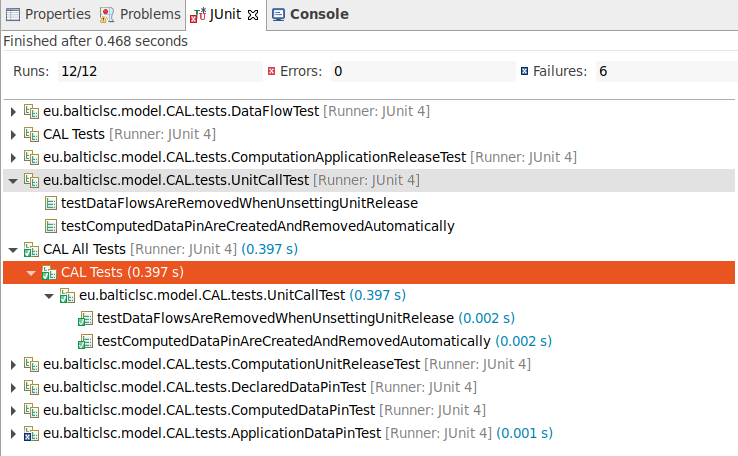
\includegraphics[width=0.95\linewidth]{./images/sirius-desktop-metamodel-tests.png}
	\caption{Wynik uruchomienia testów automatycznych
  metamodelu}\label{rys:sirius-desktop-metamodel-tests}
\end{figure}
% \end{noindent}
